\subsection{Timing Attacks}
Timing attacks are a class of side-channel attacks that exploit the fact that the execution time of a program can depend on the input.
The history of timing attacks goes back several decades where Kocher showed multiple successful timing attacks on well-known cryptographic algorithms such as Diffie-Hellman and RSA \citep{1996-timing-attacks}.
An example of vulnerable code is shown in Figure \ref{fig:timing-attack-example}.
\begin{figure}[H]
  \begin{lstlisting}[style=defstyle,language=C, xleftmargin=6.8cm, xrightmargin=6.8cm]
int foo(int x) {
  if (x < 100) {
    x *= 2;
    x += 7;
  }
  return x;
} \end{lstlisting} 
  \caption{Example of a program vulnerable to a timing attack. 
  Only by analyzing the execution time of the machine code, an attacker can infer whether the input is less than 100 or not.}
  \label{fig:timing-attack-example}
\end{figure}

\subsection{Optimizing Compilers}
Cryptographers will avoid code like the example in Figure \ref{fig:timing-attack-example} and write constant-time code instead.
Constant-time code is code where the execution time is independent of the input.
However, the compiler may introduce timing vulnerabilities through optimizations by adding variable-time branches to the machine code.
The issue arises in the analysis and transformation phases of the compiler as illustrated in Figure \ref{fig:optimizing-compiler-pipeline}.

\begin{figure}[H]
  \centering
  \tikzstyle{box} = [rectangle, minimum width=2.8cm, minimum height=1cm, text centered, draw=black]
\tikzstyle{arrow} = [thick,->,>=stealth]

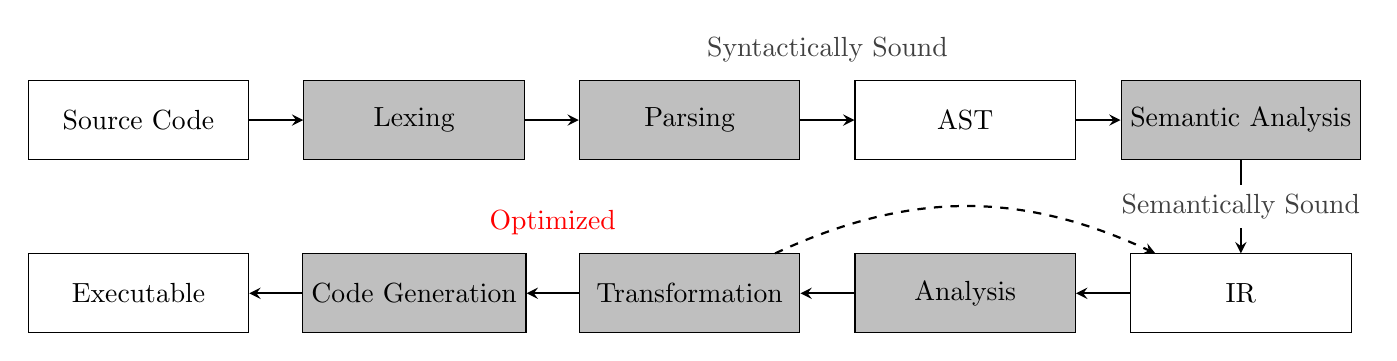
\begin{tikzpicture}
  \node (Source Code) [box] {Source Code};
  \node (Lexing) [box, fill=lightgray, right of=Source Code, xshift=2.5cm] {Lexing};
  \node (Parsing) [box, fill=lightgray, right of=Lexing, xshift=2.5cm] {Parsing};
  \node (AST) [box, right of = Parsing, xshift=2.5cm] {AST};
  \node (Semantic Analysis) [box, fill=lightgray, right of=AST, xshift=2.5cm] {Semantic Analysis};
  \node (Intermediate Representation) [box, below of=Semantic Analysis, yshift=-1.2cm, xshift=0cm] {IR};
  \node (Analysis) [box, fill=lightgray, left of=Intermediate Representation, xshift=-2.5cm] {Analysis};
  \node (Transformation) [box, fill=lightgray, left of=Analysis, xshift=-2.5cm] {Transformation};
  \node (Code Generation) [box, fill=lightgray, left of=Transformation, xshift=-2.5cm] {Code Generation};
  \node (Executable) [box, left of=Code Generation, xshift=-2.5cm] {Executable};

  \draw [arrow] (Source Code) -- (Lexing);
  \draw [arrow] (Lexing) -- (Parsing);
  \draw [arrow] (Parsing) -- node [fill=white, text=darkgray, yshift=0.9cm] {Syntactically Sound} (AST);
  \draw [arrow] (AST) -- (Semantic Analysis);
  \draw [arrow] (Semantic Analysis) -- node [fill=white, text=darkgray] {Semantically Sound} (Intermediate Representation);
  \draw [arrow] (Intermediate Representation) -- (Analysis);
  \draw [arrow] (Analysis) -- (Transformation);
  \draw [arrow, dashed] (Transformation) to [bend left=25] (Intermediate Representation);
  \draw [arrow] (Transformation) -- node [fill=white, text=red, yshift=0.9cm] {Optimized} (Code Generation);
  \draw [arrow] (Code Generation) -- (Executable);
\end{tikzpicture}
  \caption{The pipeline of an optimizing compiler. After the transformation phase, the IR is optimized and the compiler may have introduced timing vulnerabilities.}
  \label{fig:optimizing-compiler-pipeline}
\end{figure}

Many different kinds of optimization techniques are carried out by optimizing compilers, some of which can introduce timing vulnerabilities.
Some common optimization techniques like common subexpression elimination and strength reduction have been shown to introduce timing vulnerabilities \citep{optimizations-linked-to-timing-attacks}.
To illustrate this point, we look at how common subexpression elimination can introduce timing vulnerabilities.

\subsubsection{Timing Vulnerabilities Through Common Subexpression Elimination}
\label{sec:cse}
Common Subexpression Elimination is an optimization technique that extracts subexpressions that are common across multiple expressions and replaces them with a single variable.
This optimization technique can introduce timing vulnerabilities since it can decrease the number of instructions executed for a specific branch of the code as illustrated in Figure \ref{fig:common-subexpression-elimination}.
Here the common subexpression \texttt{2 * 3 + 5} is extracted and assigned to the variable \texttt{common}, making the \texttt{else} branch execute faster than the \texttt{if} branch.

\begin{figure}[H]
  \centering
     \begin{subfigure}[b]{0.3\textwidth}
        \begin{lstlisting}[style=defstyle, language=C]
int foo(int x, int *arr) {
  if (x == SECRET) {
    x = arr[0] * 3 + 5;
    x += arr[1] * 3 + 5;
    x += arr[2] * 3 + 5;
  } else {
    x = 2 * 3 + 5;
    x += 2 * 3 + 5;
    x += 2 * 3 + 5;
  }
  return x;
} \end{lstlisting} 
         \caption{Original code.}
    \end{subfigure}
    \hspace{1cm}
    \begin{subfigure}[b]{0.3\textwidth}
      \begin{lstlisting}[style=defstyle, language=C]
int foo(int x, int *arr) {
  if (x == SECRET) {
    x = arr[0] * 3 + 5;
    x += arr[1] * 3 + 5;
    x += arr[2] * 3 + 5;
  } else {
    // optimized
    int common = 2 * 3 + 5;
    x = 3 * common;
  }
  return x;
} \end{lstlisting} 
       \caption{Optimized code.}
  \end{subfigure}
  \caption{An example of how the common subexpression elimination can introduce timing vulnerabilities in code. (a) shows the original code and (b) shows the optimized code.}
  \label{fig:common-subexpression-elimination}
\end{figure}